\section{Duon current}\label{sec:duon-current}

\begin{definition}[Duon current]
A duon current is carried hinge-current through knot support. It has form
\begin{equation}
D_i\mu D_j,
\qquad
D_i,D_j\in\{D_\alpha,D_\Omega\},
\qquad
\mu\in\{-1,0,+1\}.
\label{eq:duon-current}
\end{equation}
The \(D\)-terms are oriented dion returns. The middle \(\mu\) is the carried monon hinge, seat, or pivot.
\end{definition}

The primitive resolved family has
\[
2\times 3\times 2=12
\]
variants. Duon, duad, wavelet. \apref{app:cc-duon-duad-wavelet}.

\paragraph{Duon witness of fractal tesseract topology.}
The fractal tesseract topology is generated by recursive branch/hinge/branch inheritance. A resolved duon supplies the first finite carried-current witness of that topology. Its four active dion positions give a local \(\Qfour\) chart, while the middle hinge remains the ternary fibre.

\paragraph{Tick/click form.}
Let \(K_t\) be a field-knot state. A tick emits a duon current
\[
X_t=E(K_t).
\]
A click receives a returned duon \(Y_t\). The knot update is
\[
K_{t+1}=U(K_t,Y_t,\beta_t,\Delta_{\mathrm{lead/lag}}),
\]
and the next tick emits
\[
X_{t+1}=E(K_{t+1}).
\]
Thus the field knot converts received duon current into changed emitted duon current.

\paragraph{Markovian and retained-history handoff.}
A Markovian handoff continues by present motif state. A retained-history handoff carries prior return, lead--lag burden, jitter, shell residue, duration, or PADAR channel memory. Retained-history is the AOD term for handoff whose next state follows the present state together with retained return. Both forms carry wave handoff when distinction-information persists through recurring duon-wavelet motif form.

\begin{figure}[H]
\centering
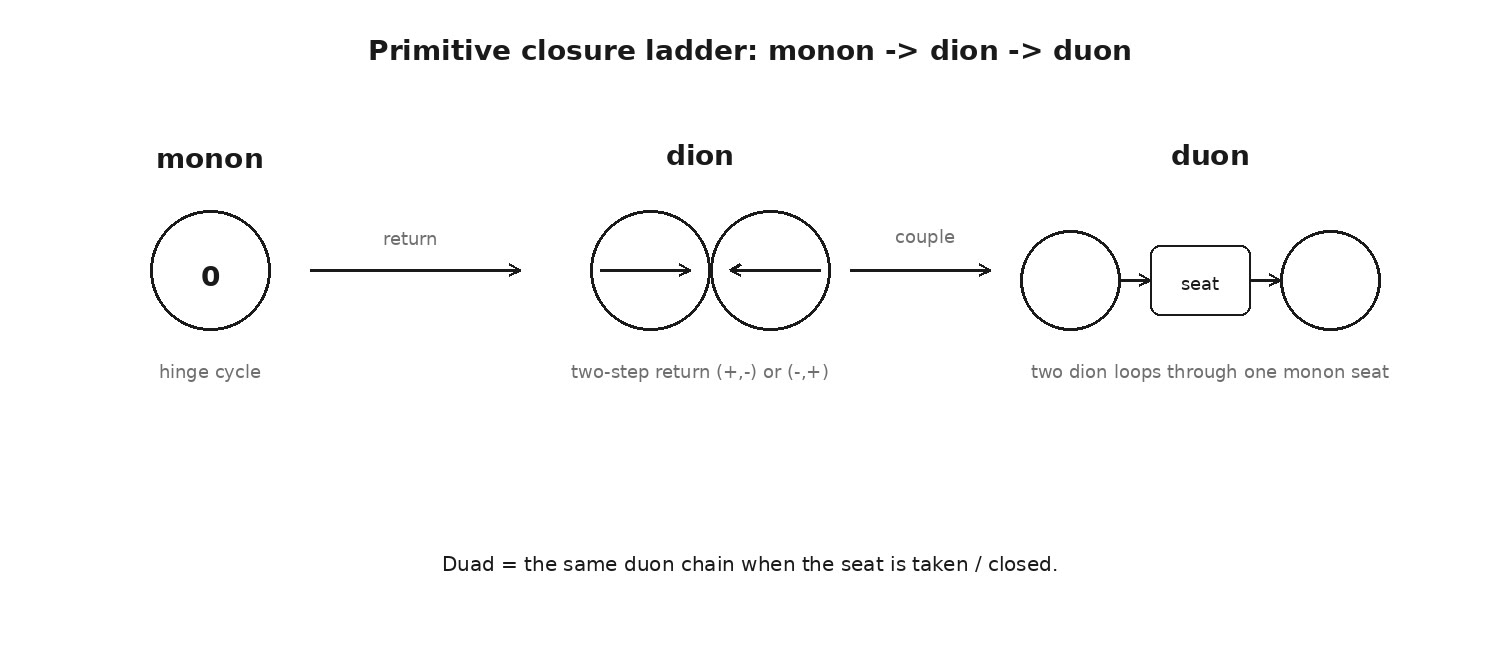
\includegraphics[width=0.84\linewidth]{figures_jpg/closure_ladder_monon_dion_duon_v32.jpg}
\caption{Primitive closure ladder. A monon is the hinge cycle; a dion is the first two-position return; a duon is two dion returns coupled through one carried monon seat. A duad is the seat-taken state of the same current.}
\label{fig:closure-ladder}
\end{figure}
